% Created 2021-11-10 Wed 02:46
% Intended LaTeX compiler: pdflatex
\documentclass[a4paper]{article}
\usepackage[utf8]{inputenc}
\usepackage[T1]{fontenc}
\usepackage{graphicx}
\usepackage{grffile}
\usepackage{longtable}
\usepackage{wrapfig}
\usepackage{rotating}
\usepackage[normalem]{ulem}
\usepackage{amsmath}
\usepackage{textcomp}
\usepackage{amssymb}
\usepackage{capt-of}
\usepackage{hyperref}
\documentclass{article}
\usepackage{here}
\usepackage{xcolor}
\usepackage[margin=3.0cm]{geometry}
\usepackage{amsmath}
\usepackage{parskip}
\renewcommand\arraystretch{1.4}
\usepackage[margin=1in]{geometry}
\usepackage{minted}
\usepackage{multicol}
\definecolor{bg}{rgb}{0.95,0.95,0.95}
\newminted{java}{fontsize=\footnotesize,frame=single,framesep=2mm}
\newminted{text}{breaklines,fontsize=\footnotesize,frame=single,framesep=2mm}
\author{Fatih Kaan Salgır - 171044009}
\date{}
\title{CSE443 - Object-Orianted Analysis \& Desing - HW 2}
\hypersetup{
 pdfauthor={Fatih Kaan Salgır - 171044009},
 pdftitle={CSE443 - Object-Orianted Analysis \& Desing - HW 2},
 pdfkeywords={},
 pdfsubject={},
 pdfcreator={Emacs 27.2 (Org mode 9.5)}, 
 pdflang={English}}
\begin{document}

\maketitle

\section*{Design Explanation}
\label{sec:org9c0643d}

\subsection*{Java FX Tile Game}
\label{sec:orgd847ebb}

\texttt{Main} class creates the factories, loads the FXML template and shows the stage.
\texttt{MainController} implements \texttt{Initializable} to initialize the Grid Pane and the Hero Pane.
For displaying tiles, \texttt{GridPanel} is used.
Every tile on the grid has a \texttt{Label}.
Event handlers are added to these labels in order to listen the user input.

Hero pane consist of labels and a progress bar placed in a vertical box.
Statusbar consist of a JavaFX's \texttt{ListView}.

\texttt{common/Util.java} stores the constants used different classes like the width \& height of the window, animation durations etc.

\subsection*{Styling}
\label{sec:org5183f97}

Most of the styling of the FX elements made using CSS stylesheet (\texttt{app.css}).
When the style needed to change, such as selecting a tile or highlighting a tile, classnames are added to the \texttt{Node} or removed from the \texttt{Node}.

\subsection*{Notes}
\label{sec:org4f6f05b}

\begin{itemize}
\item User input is disabled when the animation are running.
\item The turn stays in the user, until he/she makes a successful move. (3 tiles lined up).
\item Computer is waiting for 2 seconds before it makes a move.
\end{itemize}



\newpage
\subsection*{Synchronization \& Animations}
\label{sec:org3b82fb3}

When user selects 2 tiles, and the tiles are swapped, \texttt{cascadedMove} function calls move function recursively until the grid is cleared from lined up tiles.
\texttt{move} takes another \texttt{Thread} as an arguement to wait, to enable cascading \texttt{move} calls.
\texttt{waitAndRun} function first waits for the given thread to terminate by calling \texttt{Thread.join()}, runs the runnable and, sleeps for given miliseconds.

Every step of a move runs in a seperate thread to make the steps wait for each other before running.

Steps:
\begin{itemize}
\item wait for swap
\item highlight matches
\item remove matches
\item fill gaps
\item spawn new tiles
\end{itemize}

According to JavaFX the user interface cannot be directly updated from a non-application thread.
Therefore UI updates made by the seperate thread wrapped up with \texttt{Platform.runLater(() -> \{\})}.

\texttt{move} function in the \texttt{Grid.java};

\begin{javacode}
public Thread move(Thread waitFor, boolean isSwap) {
  boolean noMatch = !matchingTiles(t -> true);
  Thread swapWait = waitAndRun(null, () -> {
  }, Util.SWAP_DURATION);
  Thread highlight = waitAndRun(isSwap ? swapWait : null, () -> {
    highlighted = matchingTiles(TileView::highlight);
  }, noMatch ? 0 : Util.HIGHLIGHT_DURATION);

  Thread scaleDown = waitAndRun(highlight, () -> {
    // remove status
    Platform.runLater(() -> statusBar.getItems().clear());
    if (highlighted) {
      performDamage(characters, enemies);
      removeHighlight();
      removeMatchingTiles();
      // update ui
      Platform.runLater(() -> enemies.asList().forEach(HeroView::updateView));
    }
  }, noMatch ? 0 : Util.SCALE_DURATION);

  Thread fillGaps = waitAndRun(scaleDown, () -> {
    fillGaps();
  }, noMatch ? 0 : Util.FILL_GAPS_DURATION);

  Thread spawnNewTiles = waitAndRun(fillGaps, () -> {
    spawnNewTiles();
    if (highlighted) {
      changeTurn();
    } else {
      userInputEnabled = true;
    }
  }, noMatch ? 0 : Util.FILL_GAPS_DURATION);

  waitAndRun(waitFor, () -> {
    swapWait.start();
    highlight.start();
    scaleDown.start();
    fillGaps.start();
    spawnNewTiles.start();
  }, 0).start();
  return spawnNewTiles;
}
\end{javacode}



\newpage
\subsection*{Abstract Factory Pattern}
\label{sec:orge6c3308}

\texttt{HeroFactory} is the abstract factory interface, and there are 3 concreate factories which are \texttt{ValhallaFactory}, \texttt{AtlantisFactory}, and \texttt{UnderwildFactory} implements the \texttt{HeroFactory}.
Factories have 3 methods in order to create heros according to type.
Factory methods call the constructor of the \texttt{Hero} with given factor values to calculate styled properties.

General damage is calculated in \texttt{Hero.java}, and styled (multiplied by 2 or 0.5) in extended hero classes.



\begin{center}
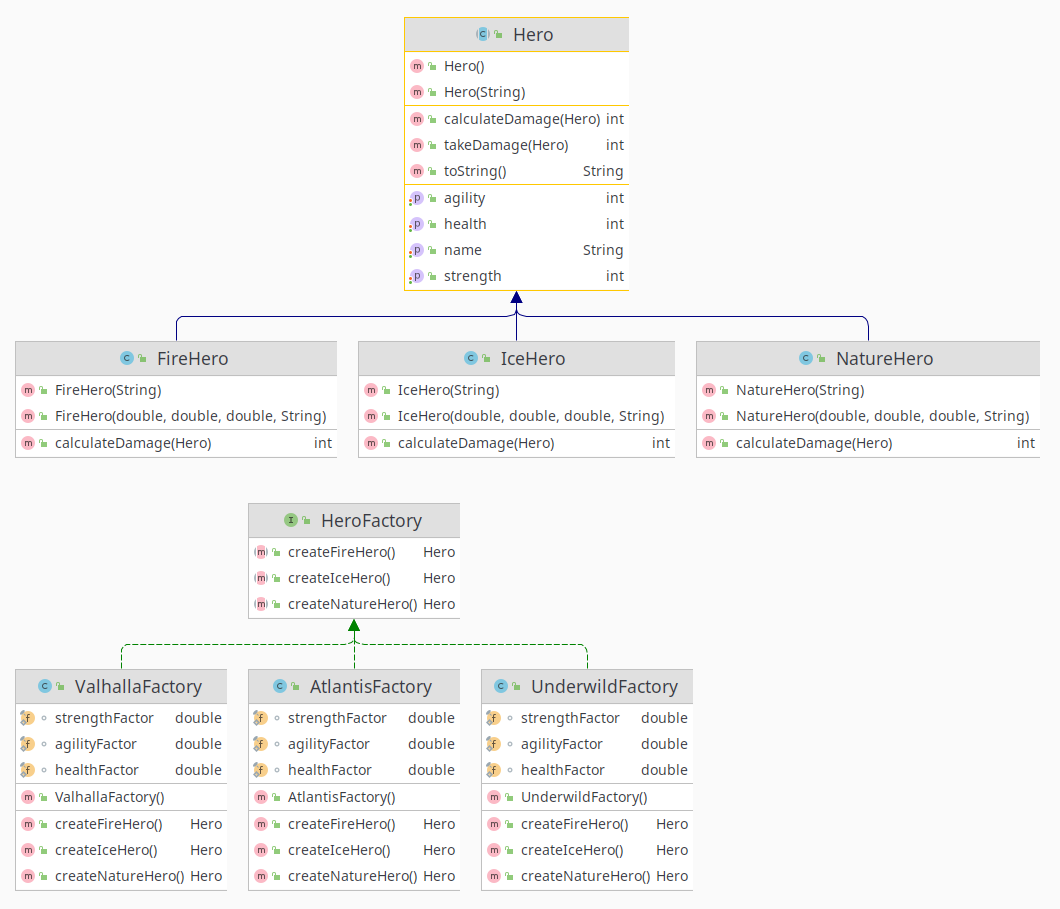
\includegraphics[width=.9\linewidth]{org-img/Design_Explanation/2021-11-09_15-45-09_screenshot.png}
\end{center}


\newpage
\subsection*{General Class Diagram}
\label{sec:org899f246}


\begin{center}
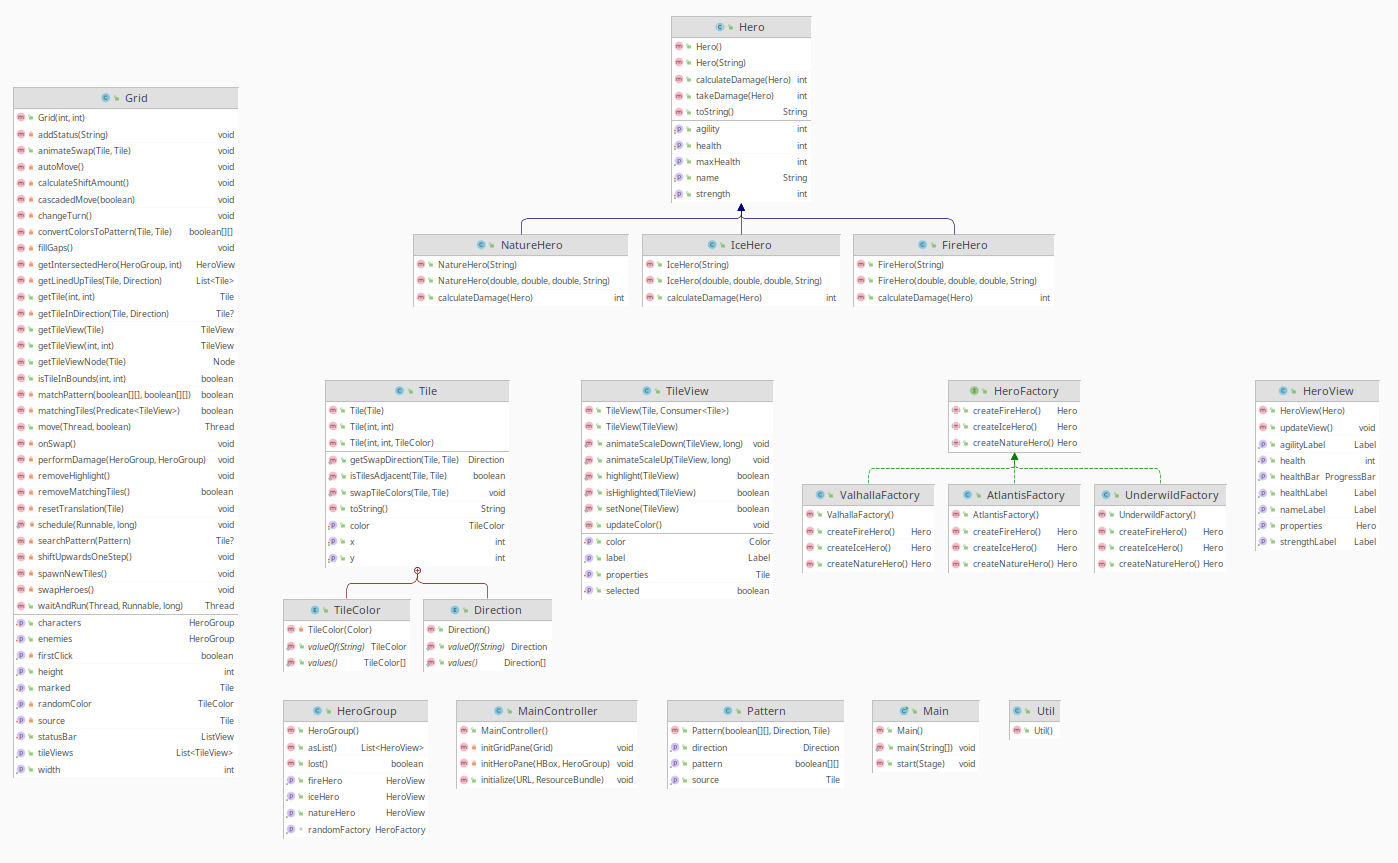
\includegraphics[width=.9\linewidth]{org-img/Design_Explanation/2021-11-10_01-49-35_screenshot.png}
\end{center}
\end{document}
